\documentclass[12pt, oneside]{article}   	% use "amsart" instead of "article" for AMSLaTeX format

%%%%%%%%%%%%%%%%%%%%%%%%%%%%%%%%%%%%%%%%%%%%%%%%%%%%
% set up packages, geometry
%%%%%%%%%%%%%%%%%%%%%%%%%%%%%%%%%%%%%%%%%%%%%%%%%%%%
\usepackage{geometry, textcomp, amsmath, graphicx, amssymb,fancyhdr,subcaption,bm}                
	
\geometry{letterpaper, marginparwidth=60pt}                   		
\usepackage[superscript,noadjust]{cite} % puts dash in citations to abbreviate
%\usepackage [autostyle, english = american]{csquotes} % sets US-style quotes
%\MakeOuterQuote{"} % sets quote style
          
\usepackage{lineno}
\usepackage{pdfpages}
\usepackage{etoolbox}
\usepackage{float,color}


\usepackage{soul}

\begin{document}

\section*{Figures}

 \begin{figure}[!h]
   \centering
       %\includegraphics[page=1,width=1\textwidth]{../../manuscript/figures/seed-bag-figure.pdf}  
       \includegraphics[page=1,width=1\textwidth]{seed-bag-figure.pdf}  
    \caption{ Summary of the seed bag burial experiments and viability trials. \hl{Figure will be labeled as (A: seed bag trials , B: viability trials, C: germination probability, D: survival probability. }. (A) The gray panel contains a graphical representation of the seed bag trials. Seeds were buried at the start of each experiment (100 seeds in month 0). Seed bags were unearthed and intact seeds ($y_{\cdot \cdot}$) and germinants ($y_{\mathrm{g},\cdot}$ counted. The graph below the panel shows a hypothetical survival function associated with persistence of seeds in the soil seed bank. (B) The gray panel contains a graphical representation of the viability trials. Seeds were tested in two rounds; germination trials were performed and then some or all of the ungerminated seeds were tested for viability. The graph below the panel shows hypothetical data from a series of viability trials and the interpolated, inferred viabilities at times when viability was unobserved. (C) Age-specific germination probably is summarized in three ways. (D) The graph shows the survival function for persistence of seeds in the soil seed bank (black line) and the estimated discrete survival probabilities for persistence and viability of seeds (orange points). }
 \label{fig:seed-bag-experiments}
\end{figure}

\clearpage
\newpage

 \begin{figure}[!h]
   \centering
       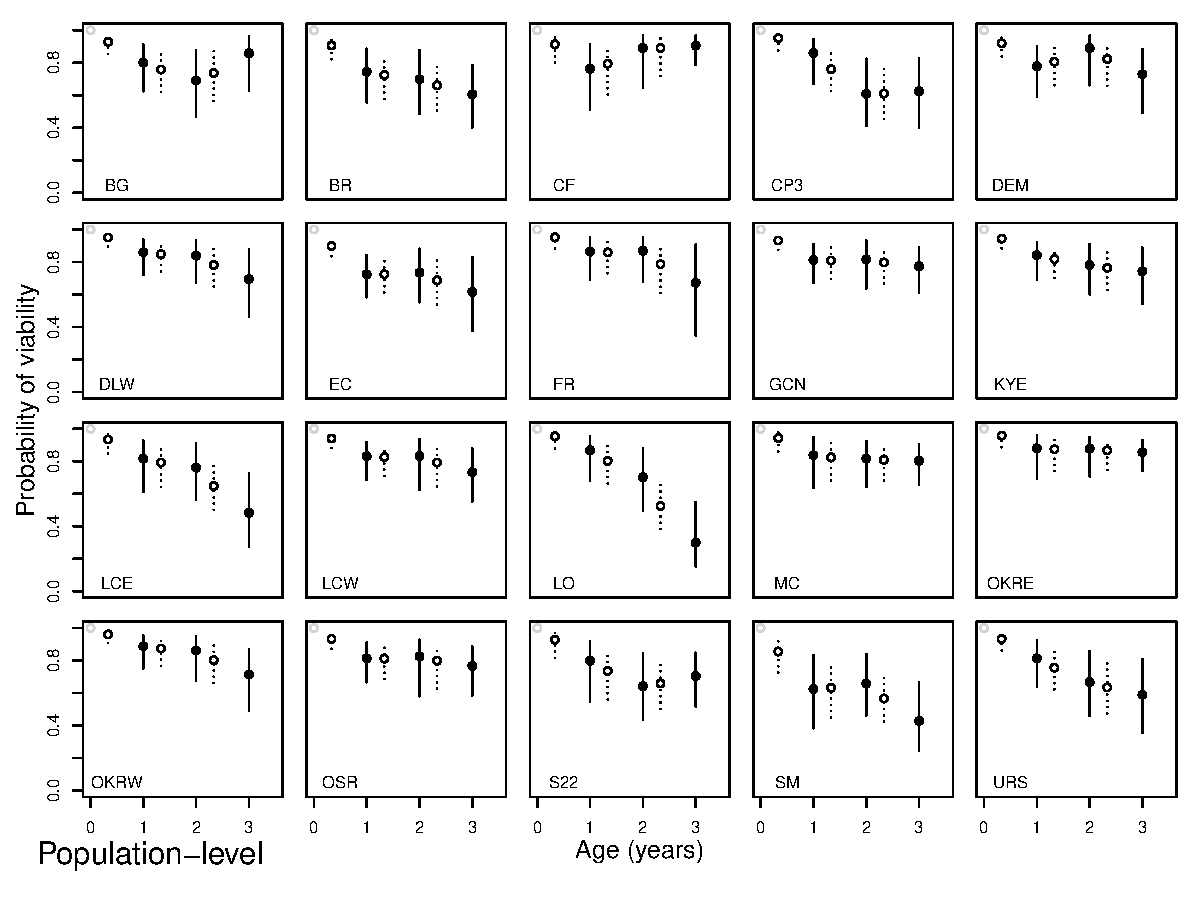
\includegraphics[page=1,width=1\textwidth]{../../figures/viability-estimates-population.pdf}  
    \caption{ Population-level estimates of viability from the 20 study populations. Filled points correspond to viability estimates from October and open points correspond to inferred viability estimates in January, interpolating between estimates as described in the main text. Points are the median of the posterior of viability; lines are the 95\% credible intervals. Three years of data contribute to estimates of viability for 1 year old seeds; two years of data contribute to estimates of viability for 2 year old seeds; one year of data contributes to estimates of viability for 3 year old seeds. }
 \label{fig:viability-estimates-population}
\end{figure}

 \begin{figure}[!h]
   \centering
       \includegraphics[page=2,width=1\textwidth]{../../figures/viability-estimates-population.pdf}  
    \caption{ Population-level estimates of median viability from the 20 study populations over three years. All populations are combined here to facilitate a visual comparison of how estimates of viability change over time across populations. Filled points correspond to viability estimates from October and open points correspond to inferred viability estimates in January, interpolating between estimates as described in the main text. Points are the median of the posterior of viability. Three years of data contribute to estimates of viability for 1 year old seeds; two years of data contribute to estimates of viability for 2 year old seeds; one year of data contributes to estimates of viability for 3 year old seeds.  }
 \label{fig:viability-estimates-population}
\end{figure}

 \begin{figure}[!h]
   \centering
       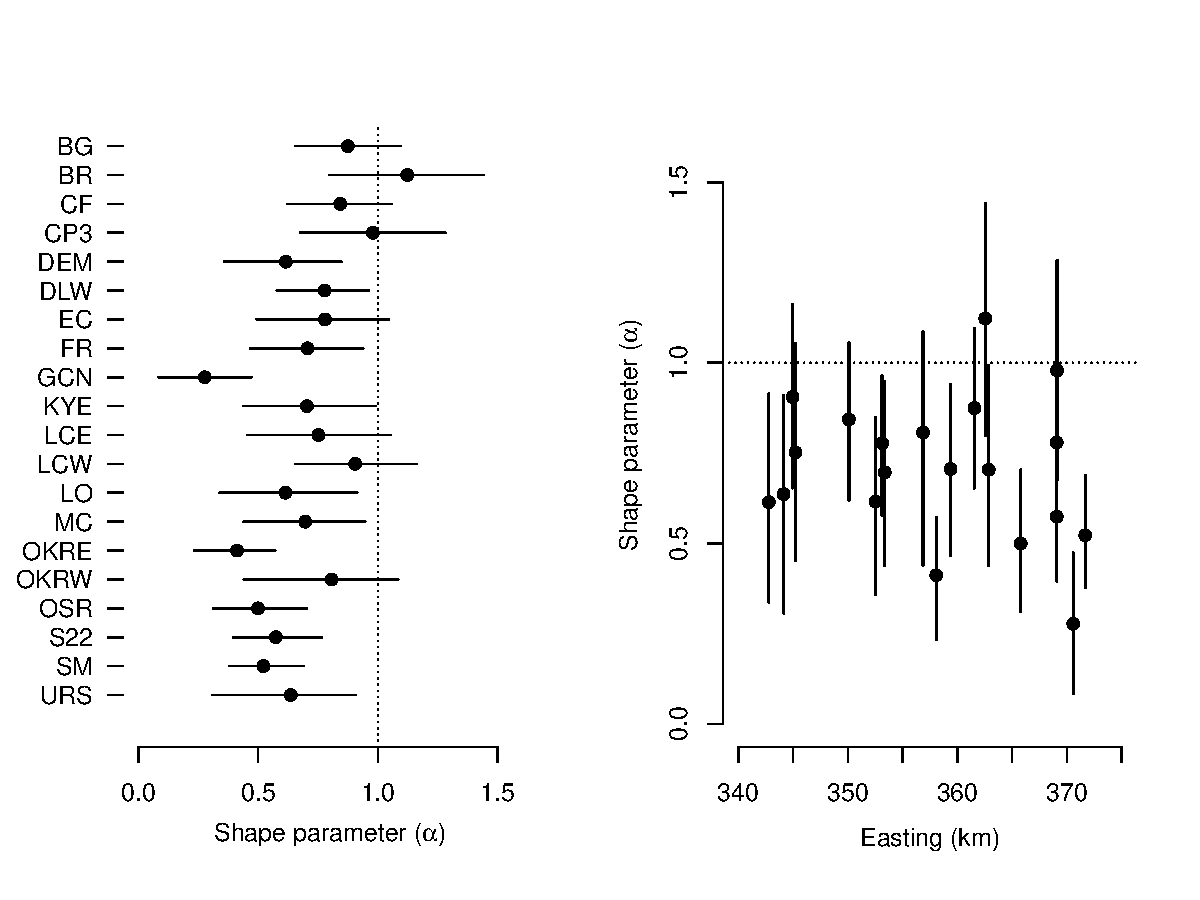
\includegraphics[page=1,width=1\textwidth]{../../figures/survival-function-parms-population.pdf}  
    \caption{ Population-level estimates for the shape parameter ($\alpha$) of the Weibull survival function. }
 \label{fig:viability-estimates-population}
\end{figure}

 \begin{figure}[!h]
   \centering
       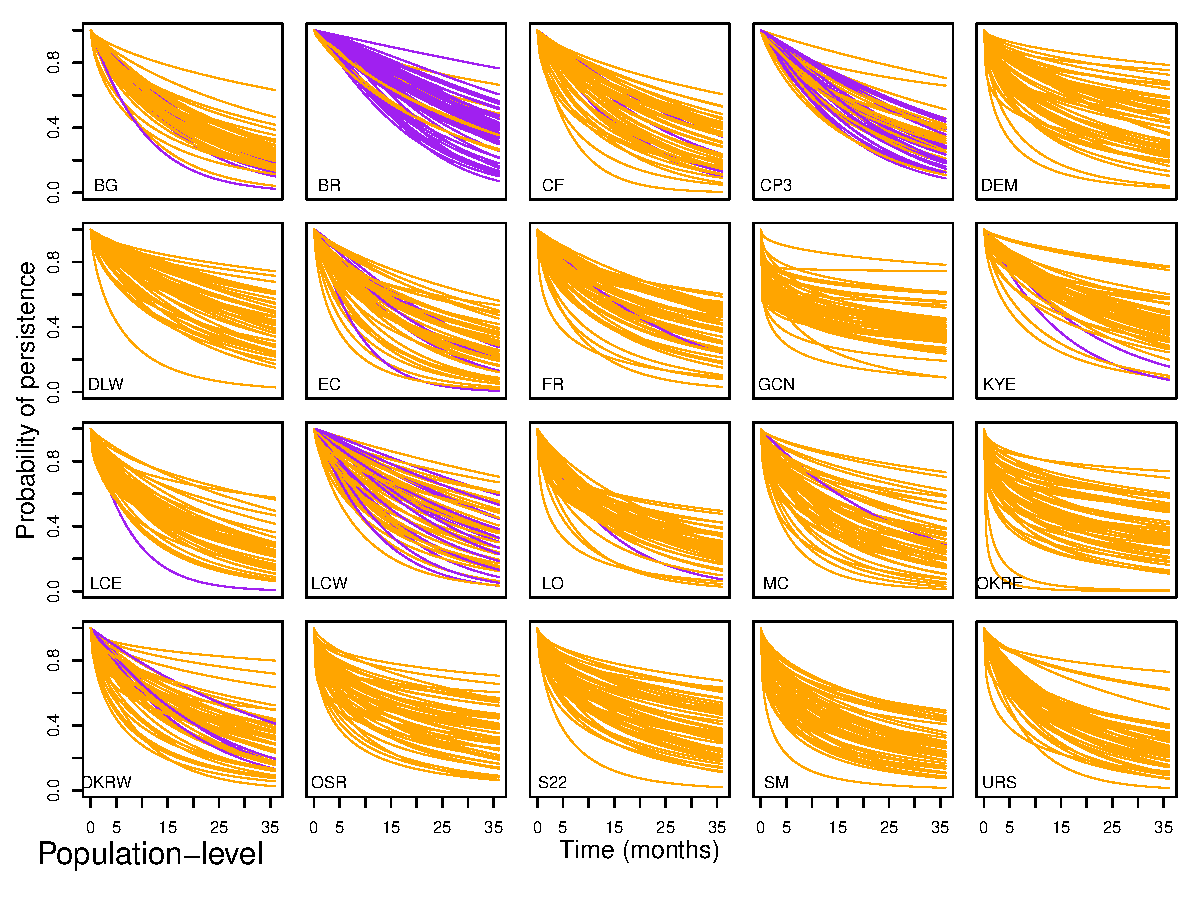
\includegraphics[page=1,width=1\textwidth]{../../figures/survival-function-population.pdf}  
    \caption{ Fifty draws from the continuous component of the population-level survival function. Each line uses one draw from the posteriors for the shape and inverse scale parameters to calculate the probability of survival  over time according to a Weibull survival function. Lines are colored so that samples for which the shape parameter is greater than one are purple, and samples for which the shape parameter is less than one are in orange.    }
 \label{fig:viability-estimates-population}
\end{figure}

 \begin{figure}[!h]
   \centering
       \includegraphics[page=2,width=1\textwidth]{../../figures/survival-function-population.pdf}  
    \caption{ The continuous component of the population-level survival function, summarized for each population by the median and 95\% credible intervals. Credible intervals were constructed by obtaining the posterior probability of survival at each time according to a Weibull survival function, and then calculating the quantiles at each time point.  }
 \label{fig:viability-estimates-population}
\end{figure}

 \begin{figure}[!h]
        \centering
        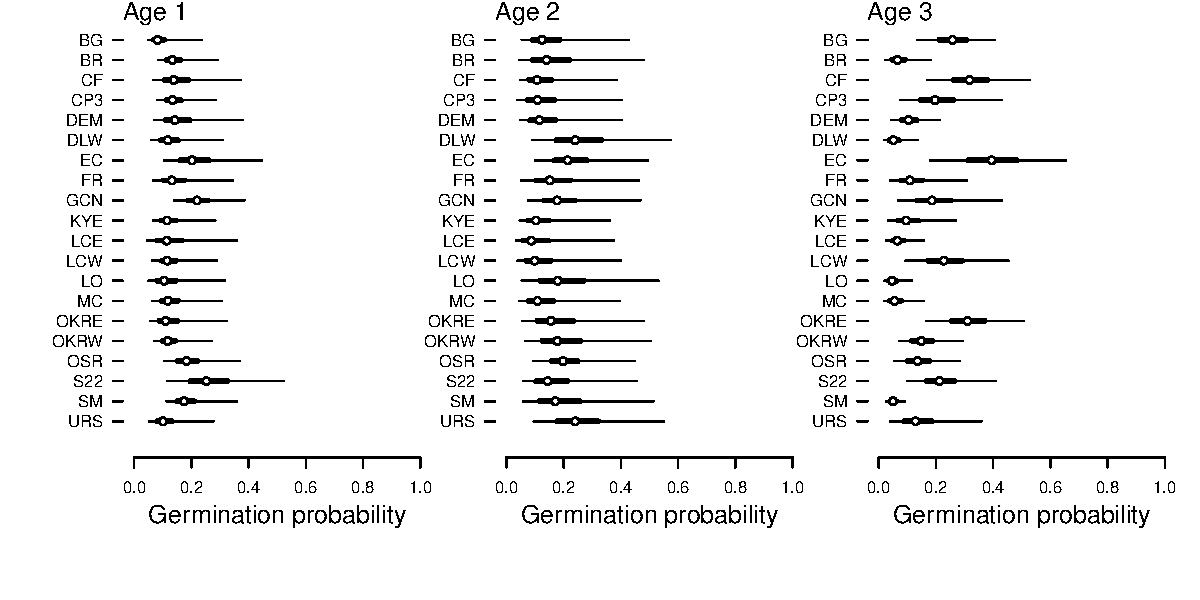
\includegraphics[page=1,width=\textwidth]{../../figures/germination-population.pdf} 
        \includegraphics[page=2,width=\textwidth]{../../figures/germination-population.pdf} 
            \caption{ The population-level probability of germination conditional on persistence. (A: top row) Age-specific germination probabilities for each population. (B: bottom row) Age-specific germination probabilities for each population plotted against the population geographic position. In all graphs, the points are the median of the posterior. Uncertainty about the estimate is summarized by the 50\% (thick line) and 95\% credible intervals (thin lines). }
 \label{fig:germination-estimates-population}
\end{figure}

 \begin{figure}[!h]
   \centering
       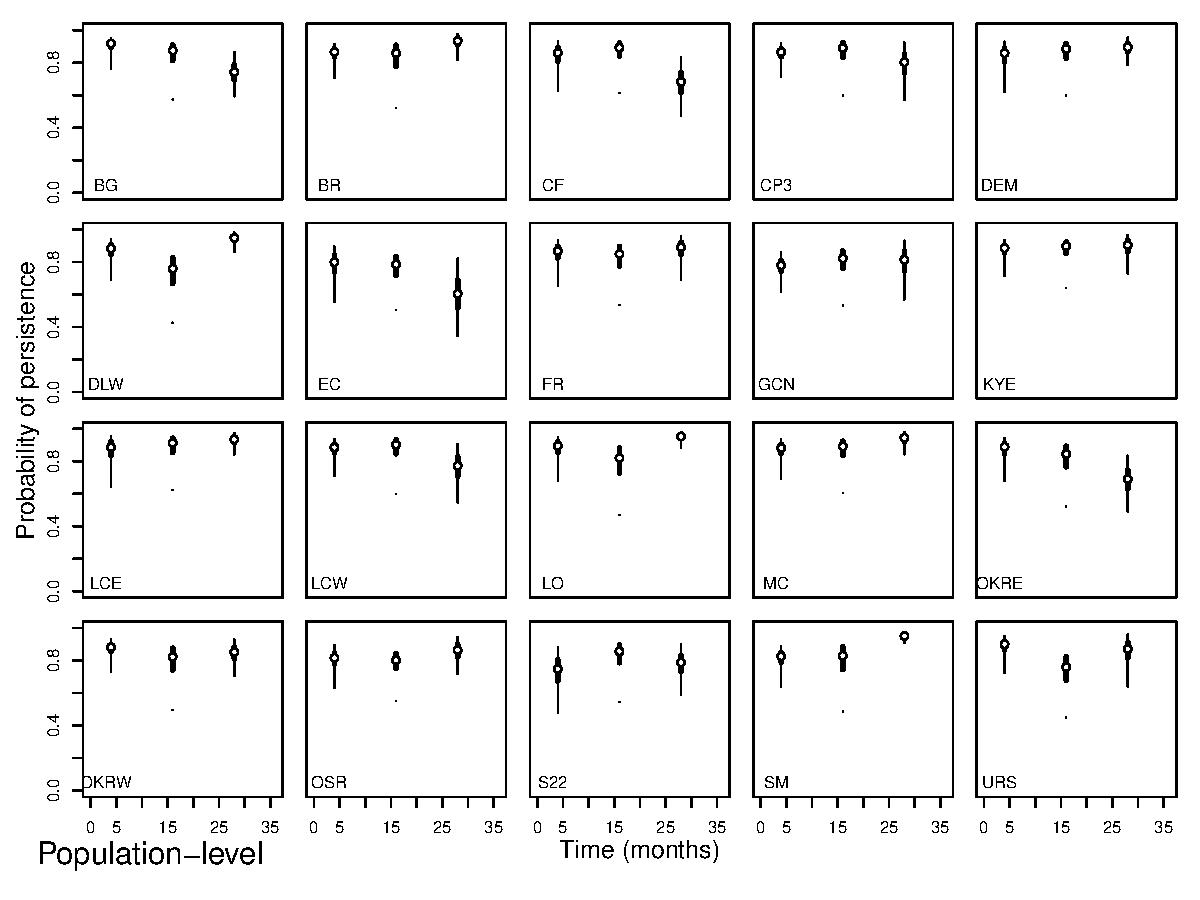
\includegraphics[page=1,width=1\textwidth]{../../figures/survival-function-discrete.pdf}  
    \caption{ The discrete component of the population-level survival function, summarized for each population by the median and 95\% credible intervals. Credible intervals were constructed by obtaining the posterior probability of persistence at each time. Times correspond to the periods at which seeds germinated; the probabilities here are the probabilities that seeds did not germinate.  }
 \label{fig:viability-estimates-population}
\end{figure}

 \begin{figure}[!h]
   \centering
       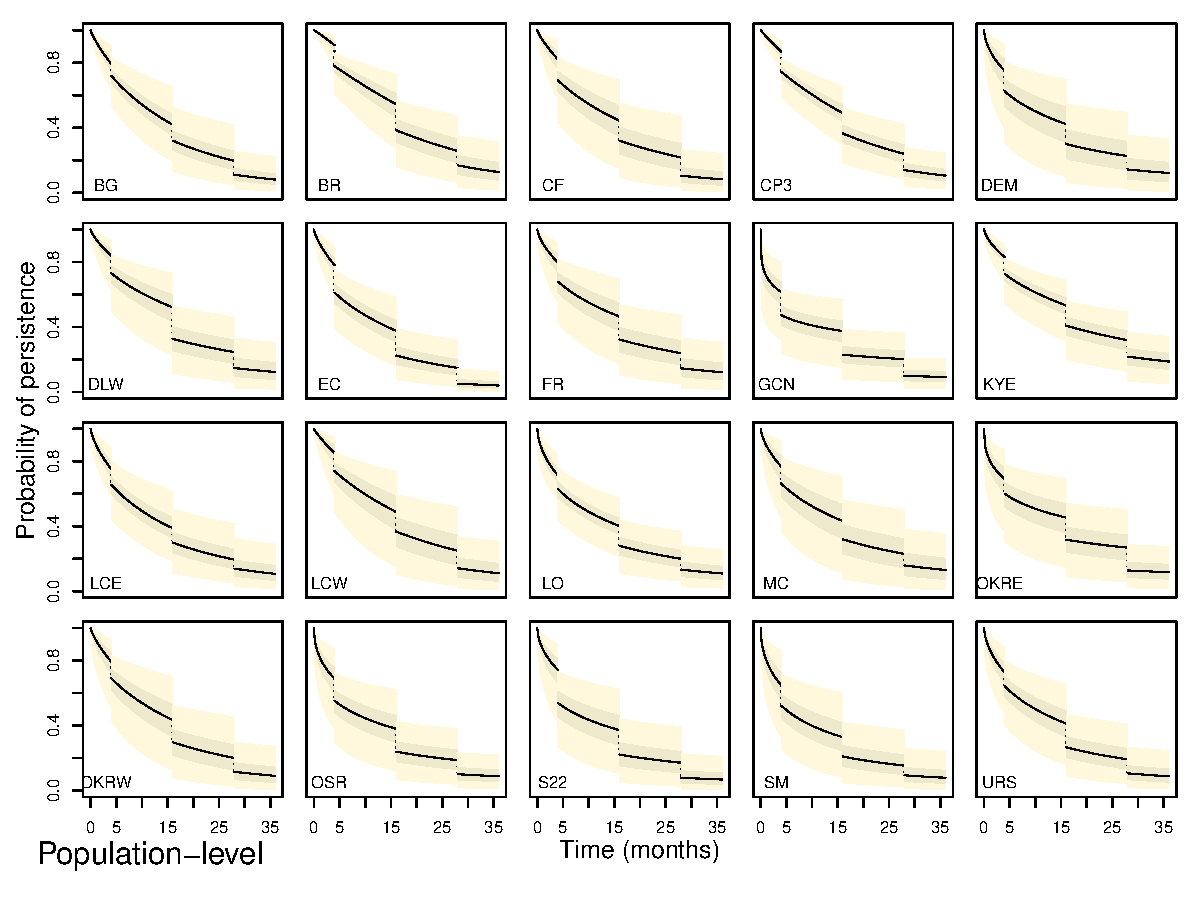
\includegraphics[page=1,width=1\textwidth]{../../figures/survival-function-compound.pdf}  
    \caption{ The combination of the continuous and discrete population-level survival function, summarized for each population by the median and 50\% \& 95\% credible intervals. Credible intervals were constructed by obtaining the posterior probability of persistence at each time. }
 \label{fig:viability-estimates-population}
\end{figure}

 \begin{figure}[!h]
   \centering
       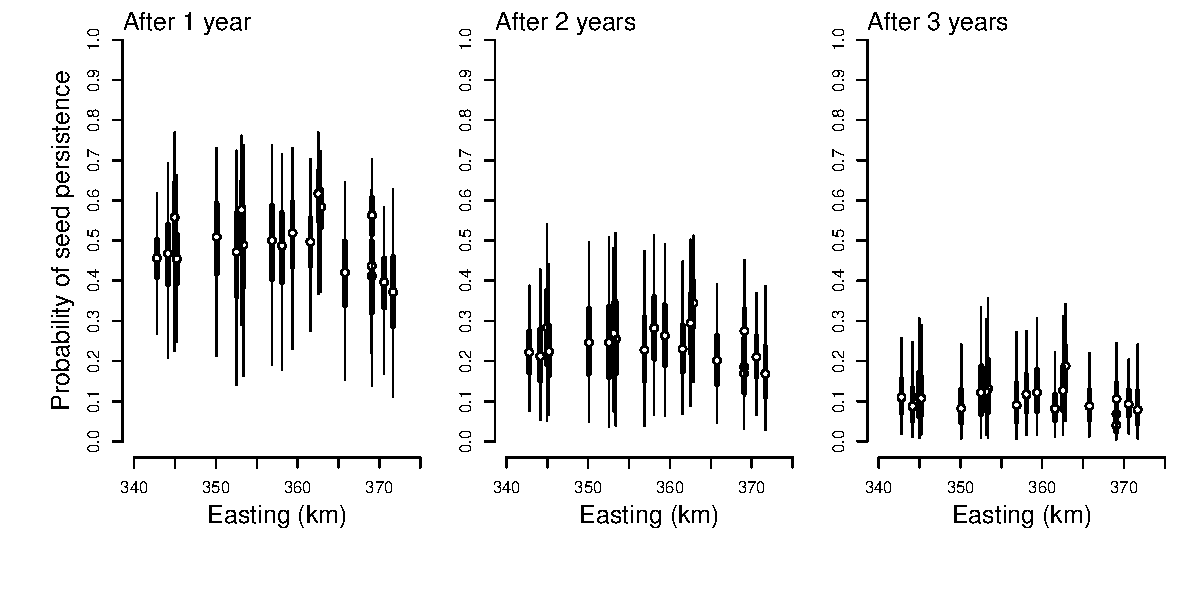
\includegraphics[page=1,width=1\textwidth]{../../figures/survival-function-summary.pdf}  
    \caption{ The population-level survival function is used to estimate the probability that seeds in each population persist after 1, 2, or 3 years in the soil. In all graphs, the points are the median of the posterior. Uncertainty about the estimate is summarized by the 50\% (thick line) and 95\% credible intervals (thin lines). }
 \label{fig:viability-estimates-population}
\end{figure}

\end{document}